\section{The Analysis of Security and Privacy}
In this section, we presents the proofs that UPPRESSO follows the required properties of security and privacy.


\subsection{Proofs of Security}

++++

Let's review the security properties in Section~\ref{subsec:basicrequirements}, including \textbf{user identification}, \textbf{RP designation}, \textbf{confidentiality} and \textbf{integrity}. In this section, we will give the brief illustration about how UPPRESSO guarantees the security properties, while the detailed process of proof is provided in the Appendix.

\noindent\textbf{User identification.}
The RP can always derive the constant and correct account from the changing $PID_U$. That is, the $PID_{RP}$ equal to $[t]ID_{RP}$ (verified by RP), and $PID_U$ equals to $[ID_U]PID_{RP}$. The $PID_{RP}$ and $PID_U$ are protected by the IdP's signature.
Thus, an RP can always derive the constant account equal to $[ID_U]ID_{RP}$.

\noindent\textbf{RP designation.}
For an honest RP, it only accepts the identity token carrying the $PID_{RP}$ equalled with $N_UID_{RP}$, while the $N_U$ is guaranteed by IdP issued registration result. Thus, the identity proof would only be accepted by the owner of $ID_{RP}$, as it is impossible to make another RP accept it by providing a malicious $N_U$.

%The detailed process of proof is shown in Appendix.

\noindent\textbf{confidentiality.}
Based on the formal model of UPPRESSO (detailed model is shown in Appendix), we can find that, there are no events carrying honest user's identity proofs, cookies and passwords sent to other malicious entities. Thus, the confidentiality of UPPRESSO system is guaranteed.

%The detailed process of proof is shown in Appendix.

\noindent\textbf{Integrity.}
The IdP-issued proofs include the $Cert$, $RegistrationResult$ and $Token$. We can easily find that the IdP does not send the private key to any processes so that the attackers cannot obtain the private key.

%The detailed process of proof is shown in Appendix.



\subsection{Proofs of Privacy}
\label{sec:analysis}
\begin{figure*}
  \centering
  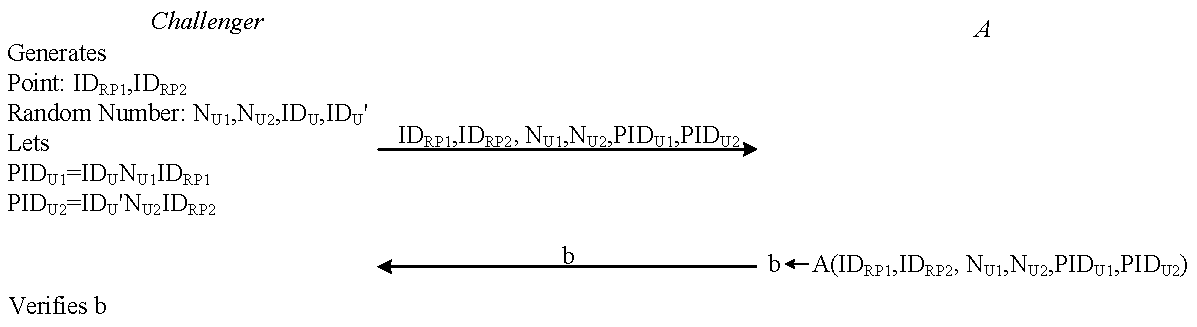
\includegraphics[width=0.82\linewidth]{fig/game1.pdf}
%  \vspace{-6mm}
  \caption{The Game.}
  \label{fig:game}
%\vspace{-7mm}
\end{figure*}

\begin{figure*}
  \centering
  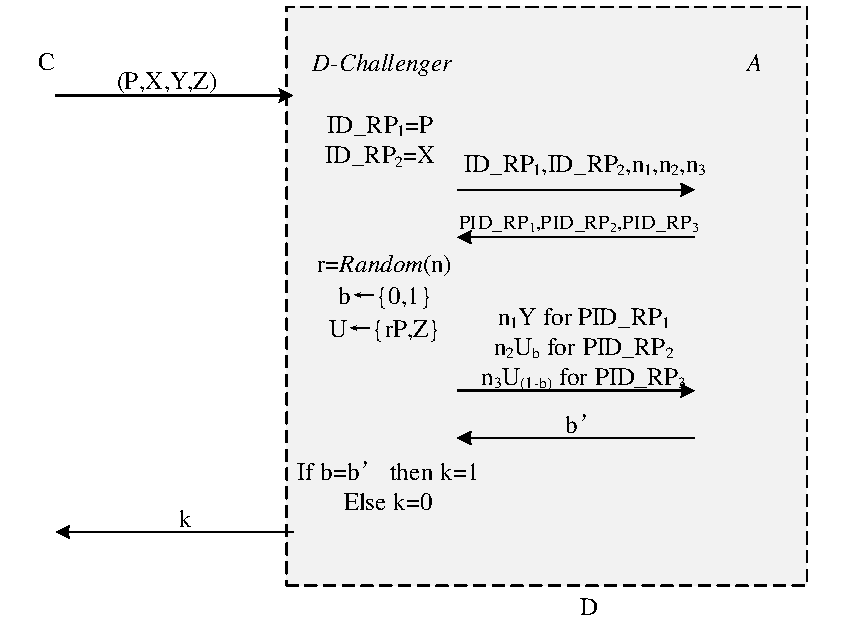
\includegraphics[width=0.65\linewidth]{fig/dalgorithm.pdf}
  \caption{The distinguishing algorithm.}
%  \vspace{-5mm}
  \label{fig:dalgorithm}
\end{figure*}
In this section, we will give the privacy proof and show that UPPRESSO is secure against both IdP-based login tracing and RP-based identity linkage attacks.

\noindent\textbf{IdP-based login tracing.}
As shown in figure~\ref{fig:process}, the only information that is related to the RP's identity and is accessible to the IdP is $PID_{RP}$,
 which is converted from $ID_{RP}$ using a random $t$.
Since $t$ is randomly chosen from $\mathbb{Z}_n$ by the user
 and the IdP has no control of the process,
 the IdP should treat $PID_{RP}$ as being randomly chosen from $\mathbb{E}$.
So, the IdP cannot recognize the RP nor derive its real identity. Therefore, IdP-based identity linkage becomes impossible in UPPRESSO.

Next, we will prove that UPPRESSO prevents RP-based identity linkage based on the Decisional Diffie-Hellman (DDH) assumption \cite{GoldwasserK16}. Here, we briefly introduce the DDH assumption:
%\noindent\textbf{The DDH Assumption.}
Let $q$ be a large prime and $\mathbb{G}$ denotes a cyclic group of order $n$ of an elliptic curve $E(\mathbb{F}_q)$.
Assume that $n$ is also a large prime. Let $P$ be a generator point of $\mathbb{G}$. The DDH assumption for $\mathbb{G}$ states that for any probabilistic polynomial time (PPT) algorithm $D$, the two probability distributions \{$aP$, $bP$, $abP$\} and \{$aP$, $bP$, $cP$\}, where $a$, $b$, and $c$ are randomly and independently chosen from $\mathbb{Z}_n$, are computationally indistinguishable in the sense that there is a negligible $\sigma(n)$ with the security parameter $n$ such that:
%where $q$ and $n$ are large primitive number, and $P$ is the point of $\mathbb{G}$.
%For any probabilistic polynomial time (PPT) algorithm $D$, the distributions, \{$P$, $aP$, $bP$, $abP$\}$_{a,b \in \mathbb{Z}_n}$ and \{$P$, $aP$, $bP$, $cP$\}$_{a,b,c \in \mathbb{Z}_n}$, are computationally indistinguishable. There is a negligible $\sigma(k)$, where $k$ is the security parameter.
\vspace{-\topsep}
\begin{multline*}
Pr[D(P, aP, bP, abP)=1]-Pr[D(P, aP, bP, cP)=1]=\sigma(n)
\end{multline*}
\vspace{-\topsep}

\vspace{-2mm}
\noindent\textbf{RP-based identity linkage.}
At the very beginning, let us see the data exposed to RP during the authentication in the UPPRESSO system.
We can find that, RP holds $ID_{RP}$,  generates $PID_{RP}$, $T$, $Account$, and receives $N_U$, registration result (containing $PID_{RP}$, hash($N_U$) and $Endpoint_U$), and identity proof (including $PID_{RP}$ and $PID_U$). Then we delete the irrelevant data, $Endpoint_U$, as it is generated randomly and does not participates and further calculation. And the repetitive data should also be deleted, for example, $PID_{RP}$ is generated as $PID_{RP}=N_U \cdot {ID_{RP}}$ so that $PID_{RP}$ can be omitted. Finally, the effective date collected by the RP during the authentication flow is $\langle ID_{RP}, N_U, PID_U\rangle$, while $PID_U$ equals to $ID_U \cdot{(N_U \cdot {ID_{RP})}}$.

%We assume that collusive can correlate $PID_U$s at different RPs and guess if they belong to the same user. Thus,
There is the data set, $\langle ID_{RP1}$, $N_{U1}$, $ID_U \cdot{(N_{U1} \cdot {ID_{RP1})}}$, $ID_{RP2}$, $N_{U2}$, $ID_U' \cdot{(N_{U2} \cdot {ID_{RP2})}}\rangle$, that RP-based identity linkage attack can be considered as RP guesses whether $ID_U$ equals $ID_U'$.
Here, we can define the game, the adversary owns the same ability as the RP. The adversary receive the input $\langle ID_{RP1}$, $N_{U1}$, $ID_U \cdot{(N_{U1} \cdot {ID_{RP1})}}$, $ID_{RP2}$, $N_{U2}$, $ID_U' \cdot{(N_{U2} \cdot {ID_{RP2})}}\rangle$ from the challenger, and returns the result $b$.
The $b$ is set 1, while adversary guess that $ID_U$ equals $ID_U'$, otherwise 0. The game is shown as Figure~\ref{fig:game}.
Therefore, whether the RP-based identity linkage attack is available is equivalent to whether adversary has the advantage on the guessing game.
We define $Pr_1$ is the probability, while the adversary returns $b=1$ as $ID_U$ equals to $ID_U'$. And $Pr_2$ is the probability, while the adversary returns $b=1$ as $ID_U$ does not equal to $ID_U'$.
Adversary has the advantage on the guessing game means that
\vspace{-\topsep}
\begin{equation}
Pr_1-Pr_2>\sigma(n)
\end{equation}
While an adversary has the advantage on the guessing game, based on the challenger and adversary, we can build a PPT distinguishing algorithm $D$ that breaks DDH assumption. The algorithm is shown as Figure~\ref{fig:dalgorithm}. That is, the input of $D$ in the form ($X$,$Y$,$Z$,$N$), while $X$,$Y$,$Z$,$N$ are points on the elliptic curve. The challenger receives the input and set $ID_{RP1}=X$, $ID_{RP2}=Y$, $PID_{U1}=N_{U1} \cdot{Z}$, and $PID_{U2}=N_{U2} \cdot{N}$.  At the end, $D$ returns the $b$ as the result.
Now, we let ($P$, $aP$, $bP$, $abP$) and  ($P$, $aP$, $bP$, $cP$) be the input. Thus there is
\vspace{-\topsep}
\begin{multline*}
\ \ \ \ \ \ \ \ \ \ \ \ \ \ \ \ \ Pr[D(P,aP,bP,abP)=1]=\\ Pr[A(P, N_{U1}, b \cdot{N_{U1}P}, aP, N_{U2},b\cdot{N_{U2} aP})=1]=Pr_1\\
Pr[D(P,aP,bP,cP)=1]=\ \ \ \ \ \ \ \ \ \
\\ Pr[A(P, N_{U1}, b \cdot{N_{U1}P}, aP, N_{U2},c/a \cdot{N_{U2}aP})=1]=Pr_2
\end{multline*}
in the first equation $ID_{U} $ and $ ID_{U}'$ all equal to $b$, while in the second equation $ID_{U}$ does not equal to $ID_{U}'$, so that
\begin{equation}
Pr_1-Pr_2=\sigma(n)
\end{equation}
There is a contradiction between equation (4) and equation (5). Therefore, an adversary cannot have the advantage on the guessing game. Thus, the RP-identity linkage attack is not available.


\begin{figure}[t]
  \centering
  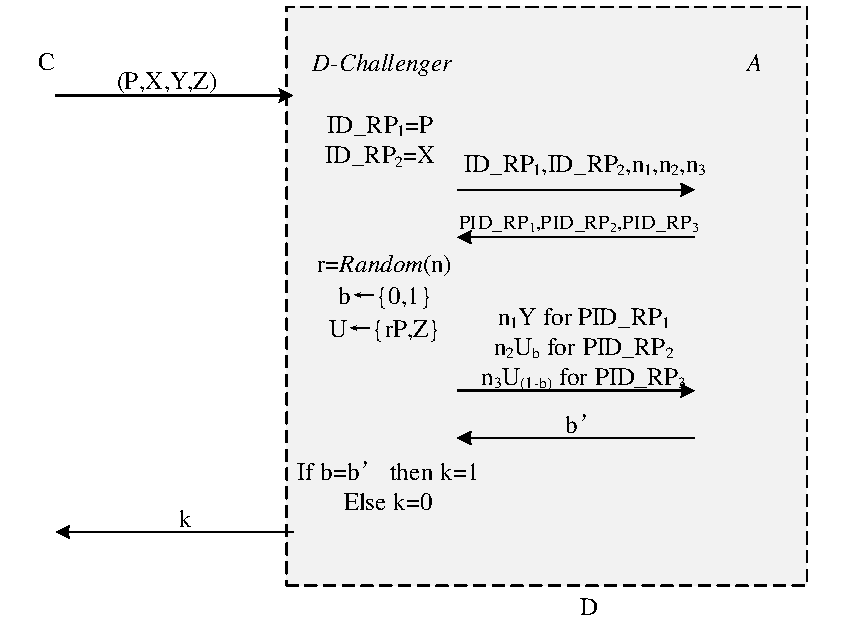
\includegraphics[width=1\linewidth]{fig/dalgorithm.pdf}
  \caption{Distinguishing algorithm.}
  \label{fig:dalgorithm}
\end{figure}
